\title{Assignment 1 \\ \small{Evolutionary Computing}}
\author{Chiel ten Brinke 3677133}
\documentclass[12pt]{article}
\usepackage{amssymb,amsmath,amsthm,enumerate,graphicx,float,lmodern,xparse}
\usepackage{hyperref}

\usepackage{tabularx,ragged2e,booktabs,caption}
\usepackage[T1]{fontenc}
\usepackage[utf8]{inputenc}
\usepackage{tabularx,ragged2e,booktabs,caption}
\newcolumntype{C}[1]{>{\Centering}m{#1}}
\renewcommand\tabularxcolumn[1]{C{#1}}
\usepackage{changepage}
%\usepackage[showframe=true]{geometry}

\newtheorem{theorem}{Theorem}[section]
\newtheorem{lemma}[theorem]{Lemma}
\newtheorem{proposition}[theorem]{Proposition}
\newtheorem{corollary}[theorem]{Corollary}

\theoremstyle{definition}
\newtheorem{definition}[theorem]{Definition}
\newtheorem{axiom}[theorem]{Axiom}
\newtheorem{example}[theorem]{Example}
\newtheorem{remark}[theorem]{Remark}

\NewDocumentCommand\set{mg}{%
    \ensuremath{\left\lbrace #1 \IfNoValueTF{#2}{}{\, \middle|\, #2} \right\rbrace}%
}

\newcommand{\co}{\texttt{counting ones}}
\newcommand{\lsco}{\texttt{linearly scaled counting ones}}
\newcommand{\tdt}{\texttt{tightly linked deceptive trap}}
\newcommand{\tnt}{\texttt{tightly linked non-deceptive trap}}
\newcommand{\rdt}{\texttt{randomly linked deceptive trap}}
\newcommand{\rnt}{\texttt{randomly linked non-deceptive trap}}

\begin{document}
\maketitle

\section{Implementation}

\subsection*{Programming language}
The algorithms have been implemented in Cython~\cite{cython}.
Cython is a programming language that makes writing C extensions for the Python language almost as easy as Python itself.
The source code gets translated into optimized C/C++ code and compiled as Python extension modules.
This allows for very fast program execution, while keeping up the high programmer productivity for which the Python language is well known.

We operate on 128 bit integers (GCC supports these), only using the first 100 bits.

\subsection*{Experiments}
Since the implemention appears to be fast enough, the number of runs that is done to decide whether a population size is successful has been doubled.
So we consider problem to be solved reliably when 58 out of 60 independent runs find the optimal solution.

To get a better idea of how the population size influences the number of successes, we do not only show the population sizes that were used during the binary search, but with intervals of 20, we show the number of successes for each population size.

However, the bisection search still has been implemented as required according to the instructions.
It has been used to determine the population size that is used to profile the fitness functions.

Other than the above, the assignment instructions have been followed precisely.
The obtained result can be found in Section~\ref{observations}.


\section{Results}
\label{observations}

\subsection*{Experiment 1}
\label{exp1}
Both randomly linked trap functions never reached an optimum.

\begin{figure}[H]
    \centering
    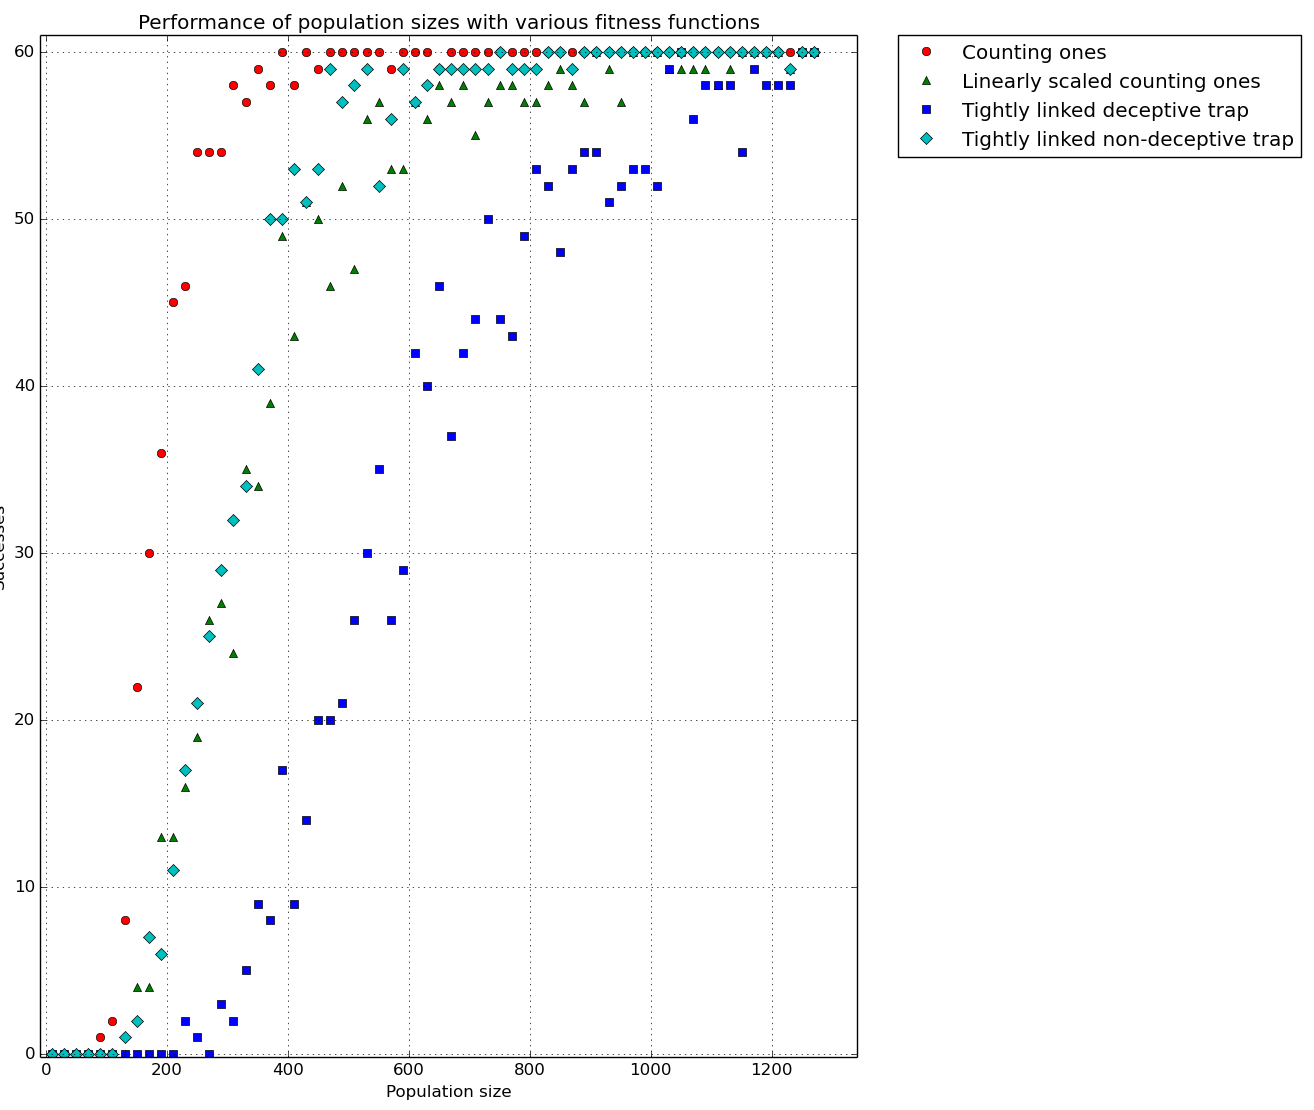
\includegraphics[totalheight=0.7\textheight]{images/exp1.png}
    \caption{Number of success per population size}
\label{fig:exp1}
\end{figure}

\begin{adjustwidth}{0cm}{}
\begin{minipage}{\linewidth}
\centering
\label{tab:title}
\begin{tabular}{lp{2.5cm}p{2.5cm}p{2.8cm}}
\toprule[1.5pt]
\bf Fitness function & \bf Population size & \bf Function evaluations & \bf Corresponding CPU time\\\midrule
Counting ones & 310 & 51094 & 0.013 seconds \\
Linearly scaled Counting ones & 730 & 164174 & 0.030 seconds \\
Tightly linked deceptive trap & 1210 & 243142 & 0.429 seconds \\
Tightly linked non-deceptive trap & 610 & 93278 & 0.177 seconds \\
\bottomrule[1.25pt]
\end{tabular}\par
\bigskip
\captionof{table}{Fitness function evaluations}
%Should be a caption
\end{minipage}
\end{adjustwidth}

% Constructs: to be expected, intuitively clear, not surprising, evident
\subsection*{Observations}
The first observation one can make is that randomly linked trap functions never reach an optimum with population sizes lower than 1280.
This is not surprising since the two-point crossover can't flip 4 bits in random places at once,
which is necessary to improve to the best state.
Unless the optimum is generated by accident at a very early stage of the evolution
(the probability of this happening is very small for the population sizes we've tried),
0s will soon dominate a lot of bit positions.
Since the two point crossover can't turn them into ones, an optimum will never be found.
% TODO: maybe mention that if a group of 4 bits are not all ones at an early stage,
% they will all converge to zero.
% The probability of a group of 4 being all 1 at once is not so big.
% The probability of every group of 4 being all 1 in at least one good state in the population
% is apparently very small
% Maybe compute this probability

We can also see that \co{} needs the smallest population size.
The two-point crossover preserves quality of good states, because if two parents have many 1s,
their offspring is also very likely to have many 1s.
Since all bits are awarded equally, it is likely that at every stage of the evolution,
every bit is set to one in some state in the population.
So that may explain the relatively low population size that is needed for the \co{} function.

The minimum required population sizes of \lsco{} and \tnt{} are not far off,
but the latter is a tiny bit lower.
It is intuitively clear why the two-point crossover needs a higher population size
with \co{} than with \lsco{}.
With \lsco{} the most significant bits contribute more to the fitness, so states with many 1s
on significant places survive better than states with many ones on insignificant places.
To make sure we don't lose the states that have the insignificant bits set to 1, we need
a population size that is big enough to ensure that every bit has a value of 1
in some state in the population.

For \tnt{}, even though all bits in a chuck (a subfunction of 4 bits) have to be turned to 1
at the same time in order to be awarded, the population size that is needed is not so big.
Apparently, the bits being 1 are not punished so hard that their states don't survive.
Instead, presumably the states with many 1s will do well, because all the chucks that
are all 1 are awarded so much, they can make up for the punishments of the remaining 1s.

% tnt vs tdt
This is not so much the case with \tdt{}.
Chucks that are all 1 are less awarded now, so states with a many 1s are punished harder
on average.
A bigger population size is needed here to make sure that 1s at all bit positions stay in the
population.
From this we could conclude that reducing deceptiveness in a fitness function
reduces the population size needed.

% Profiling
Even though \lsco{} had more function evaluations than \tnt{}, the cumulative CPU time used
is lower.
So evaluating \lsco{} is faster than \tnt{}.
And in the end the evolution finished faster as well (0.108 vs 0.240 seconds),
even though more function evaluations had to be done.
% TODO: maybe say something about (time/nr evals) ratio


\subsection*{Experiment 2}
Tightly linked deceptive trap never reached an optimum.

\begin{figure}[H]
    \centering
    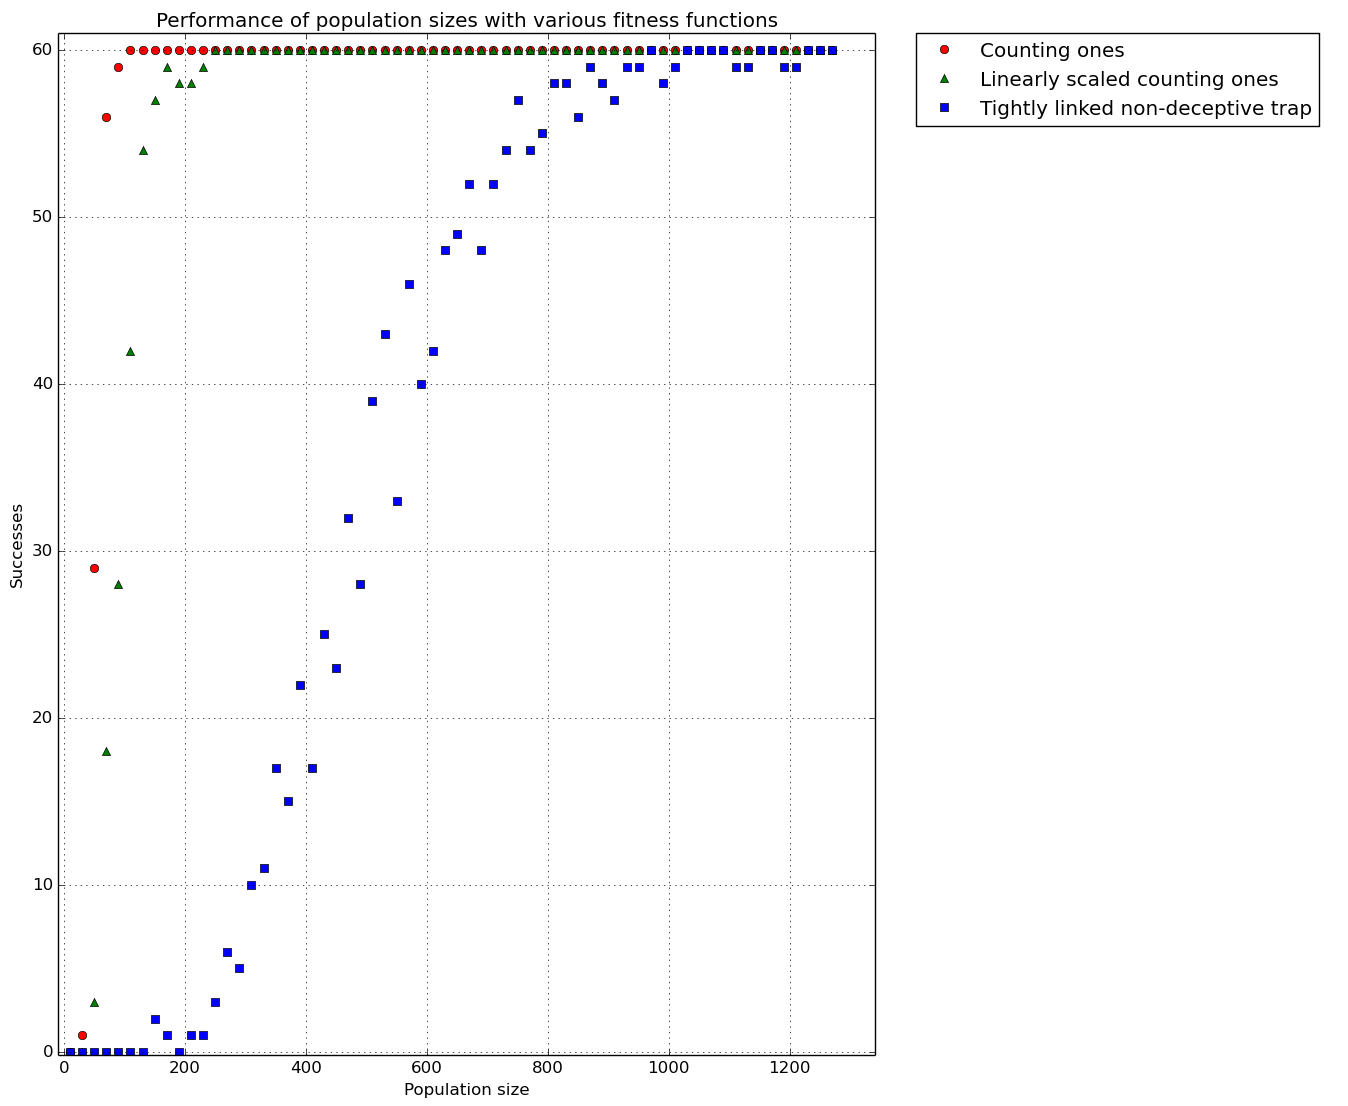
\includegraphics[totalheight=0.7\textheight]{images/exp2.png}
    \caption{Number of success per population size}
\label{fig:exp2}
\end{figure}

\begin{adjustwidth}{0cm}{}
\begin{minipage}{\linewidth}
\centering
\captionof{table}{Table Title}
\label{tab:title}
\begin{tabular}{lp{2.5cm}p{2.5cm}l}
\toprule[1.5pt]
\bf Fitness function & \bf Population size & \bf Function evaluations & \bf CPU time\\\midrule
Counting ones & 70 & 9822 & 0.002 seconds \\
Linearly scaled Counting ones & 160 & 28260 & 0.005 seconds \\
Tightly linked non-deceptive trap & 850 & 242154 & 0.454 seconds \\
\bottomrule[1.25pt]
\end{tabular}\par
\bigskip
Should be a caption
\end{minipage}
\end{adjustwidth}

\subsection*{Observations}
The first observation we make is that \tdt{} never reached an optimum.
However, in Experiment~\ref{exp1} it did.
That makes sense, because the two-point crossover is better equipped for situations where
groups of bits are interconnected w.r.t.\ to fitness.
Since this clearly is the case with \tdt{} (bits are interconnected in chunks of 4 bits),
it is not a surprise that uniform crossover needs a larger population size than
two-point crossover.

We can make a similar observation for \tnt{}, since here the populationsize needed is also
significantly larger than with Experiment~\ref{exp1}.

On the other hand, \co{} and \lsco{} need a much smaller population size than in
Experiment~\ref{exp1}.
This makes sense, because with these fitness functions there is no structure between bits.
The uniform crossover doesn't take any of such structure into account, it only looks at
individual bits.

A last remark we can make, is that for the uniform crossover randomly linkedness is the same
as tighly linkedness, since it only looks at individual bits.
Therefore, while it may seem to perform worse on the trap functions, we must not forget
that the uniform crossover solves \rnt{} equivalently as \tnt{}.
So while the two-point crossover could't reach an optimum with \rnt{} at all,
the uniform crossover could.


\subsection*{Experiment 3}
Tightly linked deceptive trap never reached an optimum.

\begin{figure}[H]
    \centering
    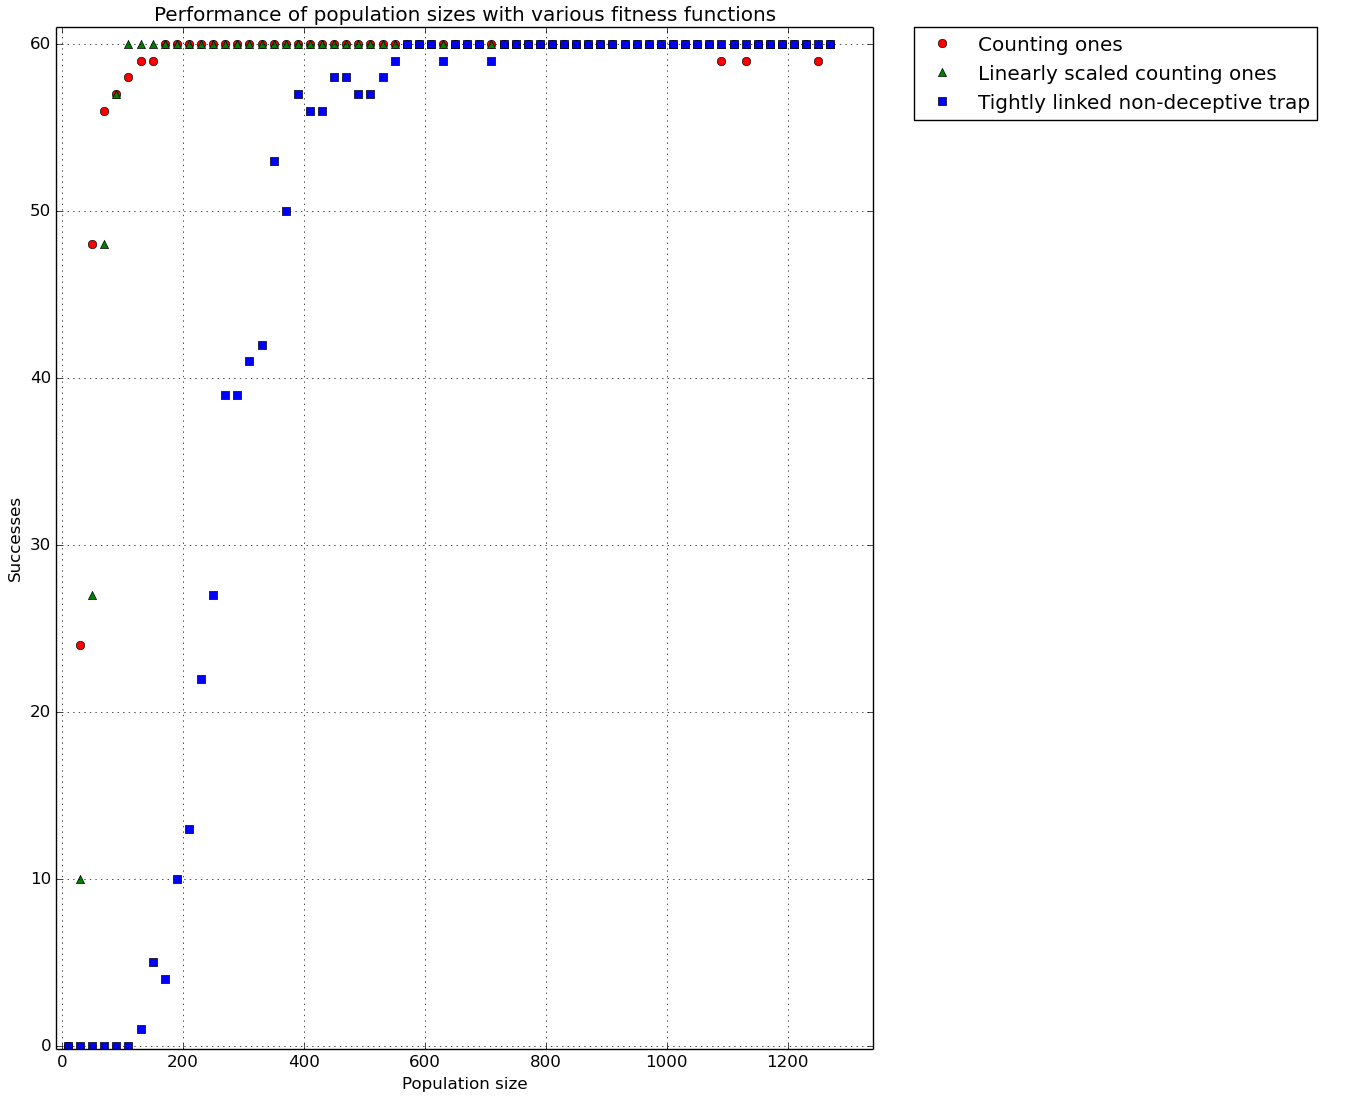
\includegraphics[totalheight=0.7\textheight]{images/exp3.png}
    \caption{Number of success per population size}
\label{fig:exp3}
\end{figure}

\begin{adjustwidth}{0cm}{}
\begin{minipage}{\linewidth}
\centering
\captionof{table}{Table Title}
\label{tab:title}
\begin{tabular}{lp{2.5cm}p{2.5cm}l}
\toprule[1.5pt]
\bf Fitness function & \bf Population size & \bf Function evaluations & \bf CPU time\\\midrule
Counting ones & 110 & 27964 & 0.007 seconds \\
Linearly scaled Counting ones & 90 & 49764 & 0.010 seconds \\
Tightly linked non-deceptive trap & 490 & 509742 & 0.582 seconds \\
\bottomrule[1.25pt]
\end{tabular}\par
\bigskip
Should be a caption
\end{minipage}
\end{adjustwidth}



\section{Conclusions}
% What kind of operators are suited for what kind of fitness functions and how this affects
% popsize and CPU time

If there is a trap in your fitness, it may help to award the optimum more,
i.e.\ make it less deceptive.

A sophisticated fitness function may perform worse than a less sophisticated function.
Even though the number of function evaluations may be less, the total computation time
may be more. See for instance \lsco{} and \tnt{}.

\begin{thebibliography}{9}

\bibitem{cython}
R. Bradshaw, S. Behnel, D. S. Seljebotn, G. Ewing, et al.,
The Cython compiler, \url{http://cython.org}.

\end{thebibliography}


\end{document}
